\subsection{\textit{Platform-independent model} (PIM)}

Considerando-se o modelo de domínio e os requisitos apresentados, identificaram-se as classes e atributos essenciais neste projeto e desenvolveu-se o diagrama de classes apresentado na figura \ref{fig:diagrama_classes}.

A classe \texttt{Home4All} constitui a \textit{facade} da camada de negócio, fornecendo uma interface simplificada para toda a lógica associada, implementada pelas restantes classes.

Salienta-se ainda o recurso muito frequentemente a associações por composição ou agregação como relações entre classes. Por exemplo, cada imóvel (\texttt{Property}) é associado a um utilizador comum (\texttt{Common}) por agregação, uma vez que estas entidades existem de forma independente, apesar de um proprietário (\textit{owner}) criar o imóvel.

Para além disso, criaram-se relações por generalização (herança) com o intuito de captar comportamento comum entre classes. Assim, um utilizador (\texttt{User}), por exemplo, poderá ser especificado num utilizador comum (\texttt{Common}) ou num administrador (\texttt{Admin}). Da mesma forma, um utilizador comum pode ser também um utilizador com conta interna, caso em que terá associada uma \textit{password}. Caso o utilizador comum se tenha autenticado com uma conta externa (Facebook ou Google), então será apenas um \texttt{Common}.

Para construir as restantes relações do diagrama de classes seguiu-se o mesmo tipo de raciocínio.

\begin{landscape}
    \begin{figure}[!ht]
        \centering
        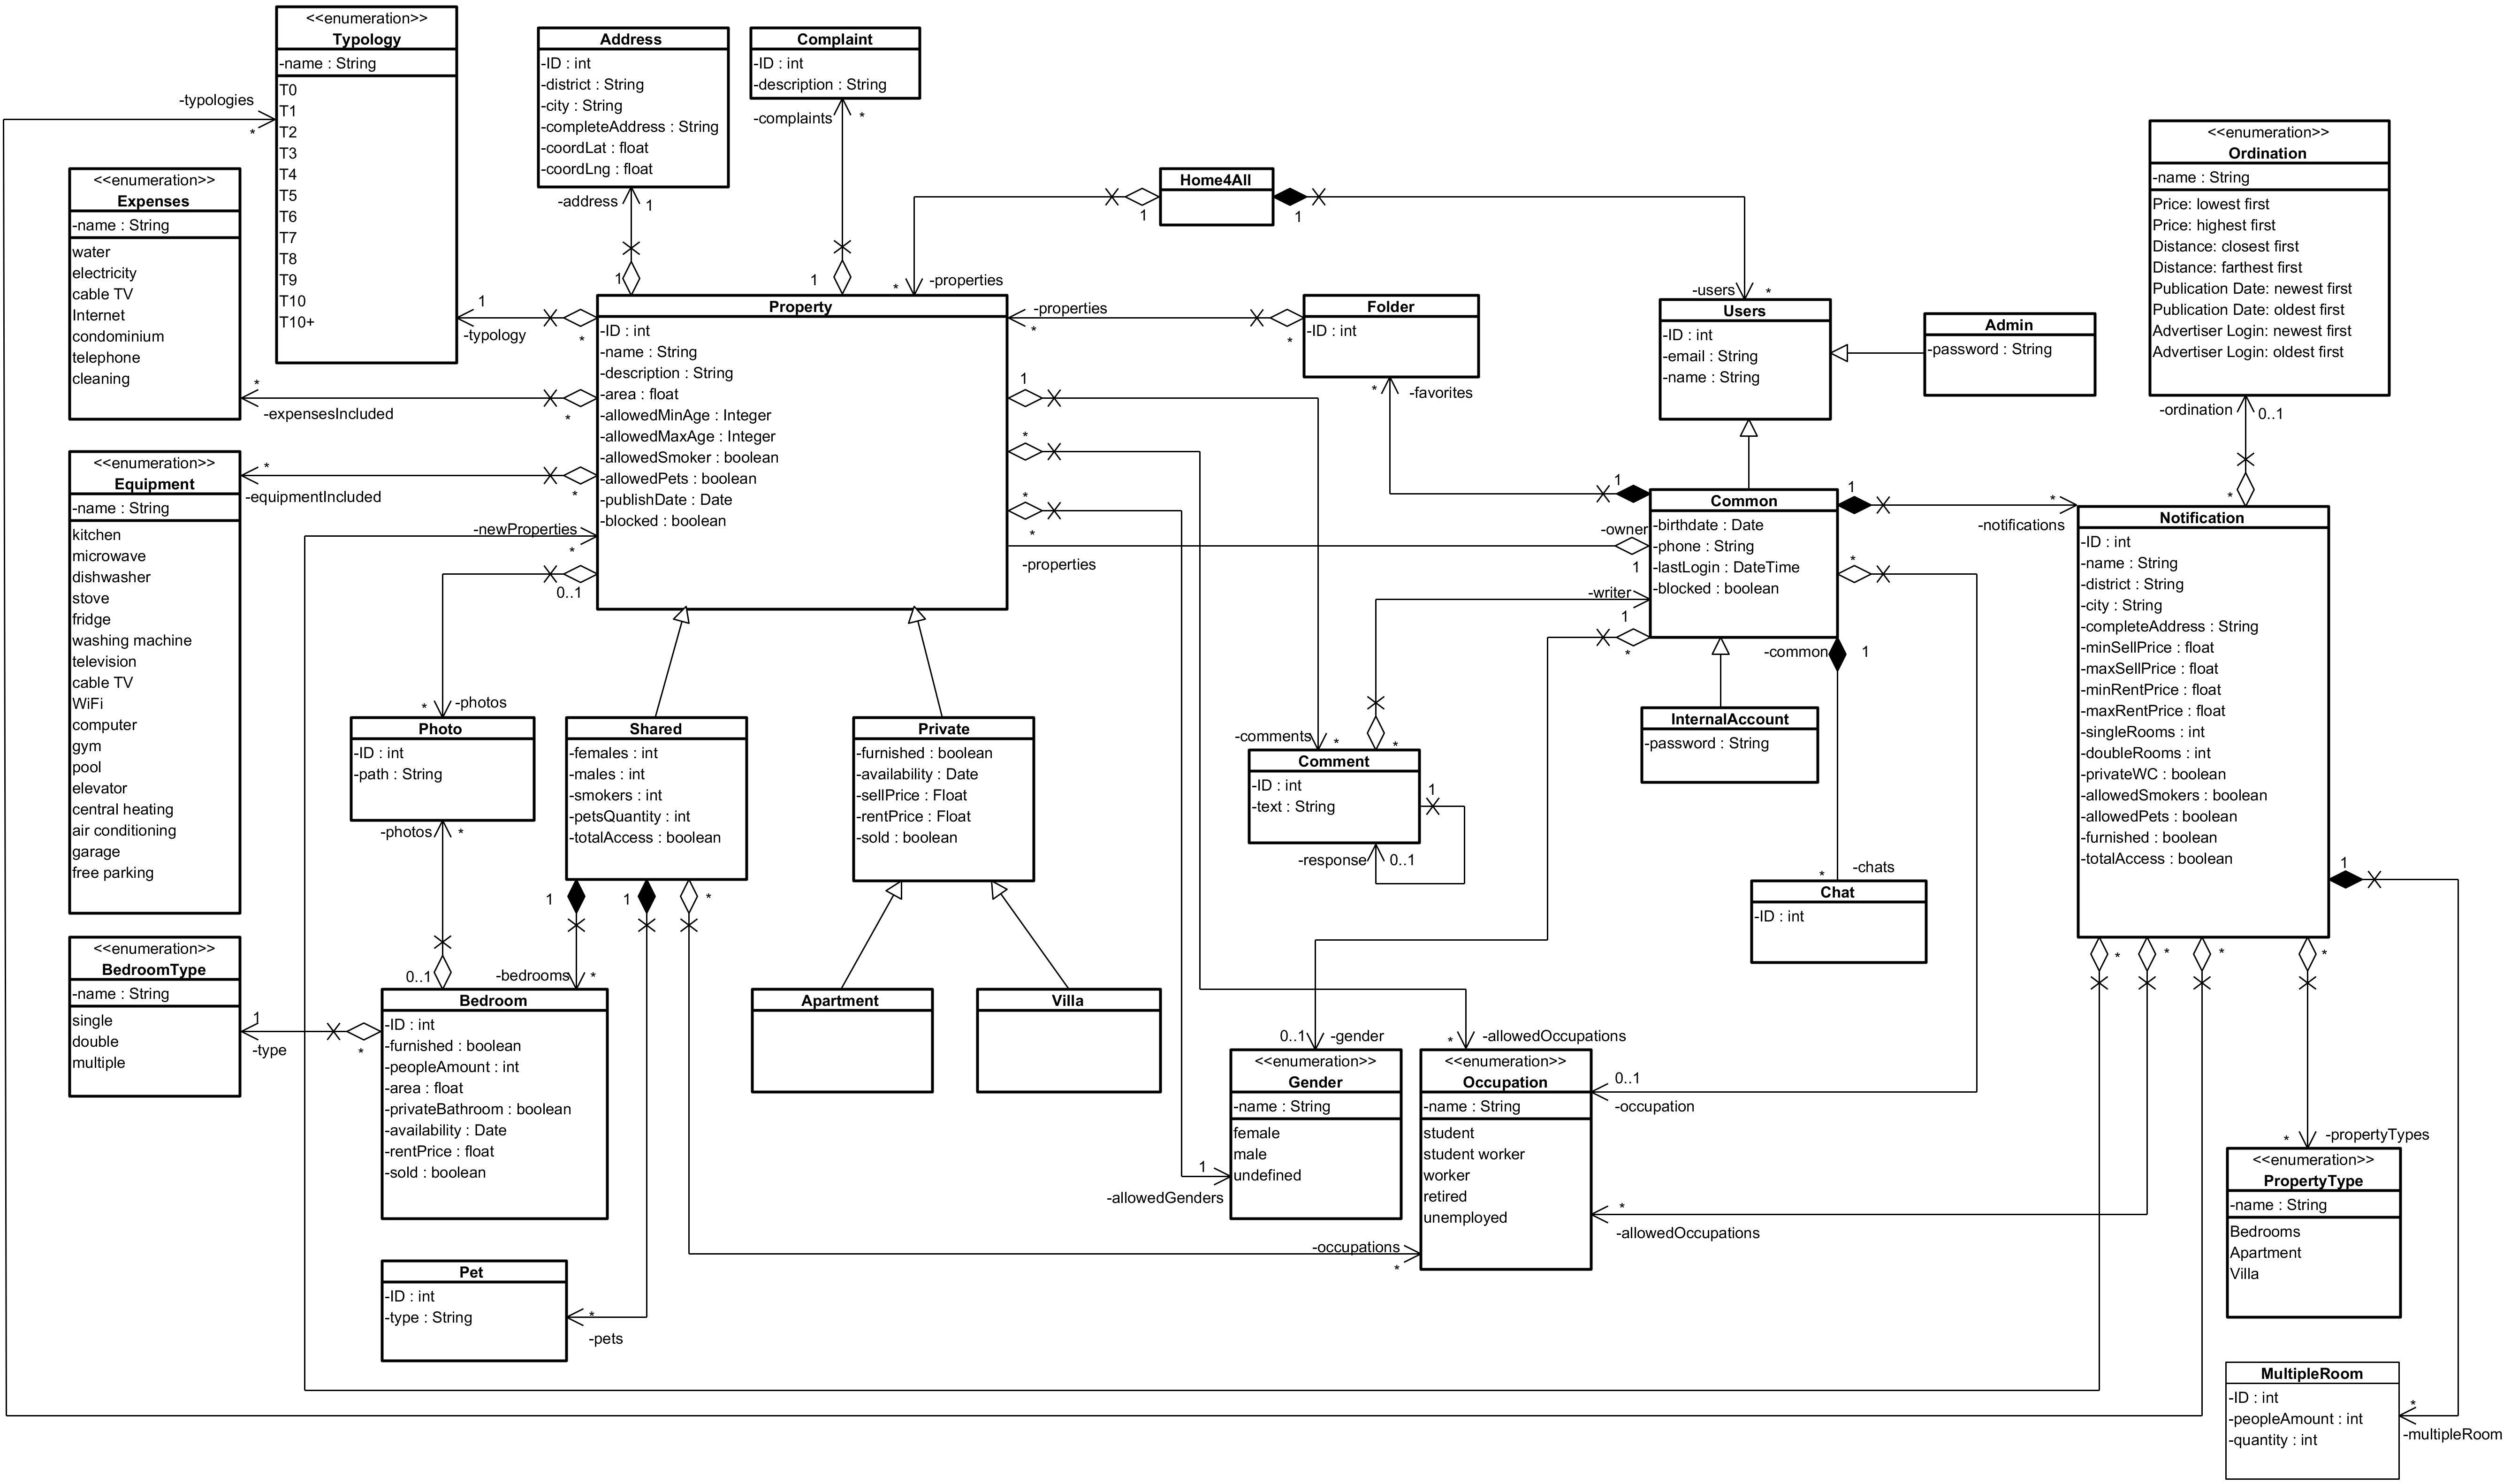
\includegraphics[width=1.6\textwidth]{images/PIM.png}
        \caption{Modelo independente de tecnologia para a aplicação \texttt{Home4All}.}
        \label{fig:diagrama_classes}
    \end{figure}    
\end{landscape}


\subsection{Escolha das tecnologias}

O projeto \texttt{Home4All} consiste na concretização de um \textit{website} relacionado com o setor imobiliário. Assim sendo, é imperativo que sejam escolhidas tecnologias que melhor se adequem ao tipo de serviço que se pretende oferecer. 

Primeiramente, tem-se a camada de apresentação, onde existem duas grandes categorias, as \textit{frameworks} que renderizam as páginas no lado do servidor (e.g. \texttt{JSP}) e aquelas que o fazem no lado do cliente (e.g. \texttt{VueJS}). No projeto \texttt{Home4All} optou-se pela segunda opção, pois esta permite uma maior reatividade, além de diminuir o número de pedidos realizados ao \textit{backend} para que este forneça a página a apresentar. Além disso, a \textit{framework} escolhida tem um número elevado de recursos já disponíveis que permitem acelerar de forma significativa o processo de desenvolvimento.

Tendo sido escolhida a tecnologia para a camada de apresentação, torna-se necessário realizar o processo equivalente para a camada de negócio. De facto, o número de opções disponíveis diminui drasticamente para esta camada. A título exemplificativo, tem-se a \texttt{framework Play!}, \texttt{Struts}, \texttt{Spring} e a plataforma JEE através de \texttt{servlets} e \texttt{Enterprise Java Beans} (EJB). Após alguma pesquisa restou a dúvida entre o \texttt{Spring} e o \texttt{JEE}. No entanto, dada a curva de aprendizagem do \texttt{Spring} e o tempo para execução do projeto, optou-se por utilizar \texttt{JEE}.

Em terceiro lugar, foi necessário escolher uma \textit{framework} para a camada dos dados. Assim como no caso da camada de negócio, também esta dispõe de um menor número de opções quando comparada com a primeira. A título exemplificativo, tem-se textit{frameworks} como o \textit{MyBatis}, \texttt{JPA} ou o \texttt{Hibernate}. Neste caso a escolha requeriu sobre a última opção uma vez que incorpora mecanismos de gestão de \textit{pool}, de \textit{cache}, de transação e, por fim, é compatível com \texttt{JEE}. 

Assim sendo, o projeto \texttt{Home4All} foi concebido utilizando \texttt{VueJS} para a camada de apresentação, \texttt{JEE} (\textit{servlets} e \textit{EJB's}) para a camada de negócio e \texttt{Hibernate} para a camada de dados.

\subsection{\textit{Platform-specific model} (PSM)}

Para especificar o diagrama de classes apresentado anteriormente, que é independente das ferramentas utilizadas (PIM), de acordo com a \textit{framework} \texttt{Hibernate}, basta aplicar o \textit{stereotype} \texttt{ORM Persistable} às entidades que se pretende persistir. Assim, obtém-se o modelo apresentado na figura \ref{fig:psm_hibernate}.

Este diagrama foi desenvolvido com a intenção de se utilizar a ferramenta \texttt{Hibernate} do \texttt{Visual Paradigm} para gerar a base de dados e o código base do projeto. Assim, houve algum cuidado adicional na construção do mesmo, de forma a evitar futuras alterações do diagrama, que implicariam a reconstrução da base de dados e do código até então desenvolvido.

Uma das principais dificuldades encontradas foi a representação das enumerações apresentadas no diagrama PIM. Pretendia-se impedir, ao nível da base de dados, que os campos relativos a enumerações tivessem valores ausentes das mesmas. Para isso, poderia utilizar-se, por exemplo, o tipo de dados \texttt{ENUM} do \texttt{PostgresSQL} para representar estas entidades. Contudo, a geração automática da base de dados a partir do diagrama não permite tal especificidade. Assim, optou-se pela solução mais semelhante a esse tipo de dados, com a criação de uma tabela para cada enumeração, com uma coluna que indica o valor da enumeração e constitui a chave primária da tabela.

Para além disso, não é possível utilizar neste diagrama tipos de dados como \texttt{Collections}, \texttt{Lists}, entre outros, para representar conjuntos de tipos básicos (como \texttt{Strings}, inteiros, etc.). Por isso, existe a necessidade de se criar objetos para esses tipos básicos no diagrama, o que motivou, por exemplo, a criação das classes \texttt{Photo} e \texttt{Pet}.

\begin{landscape}
    \begin{figure}[!ht]
        \centering
        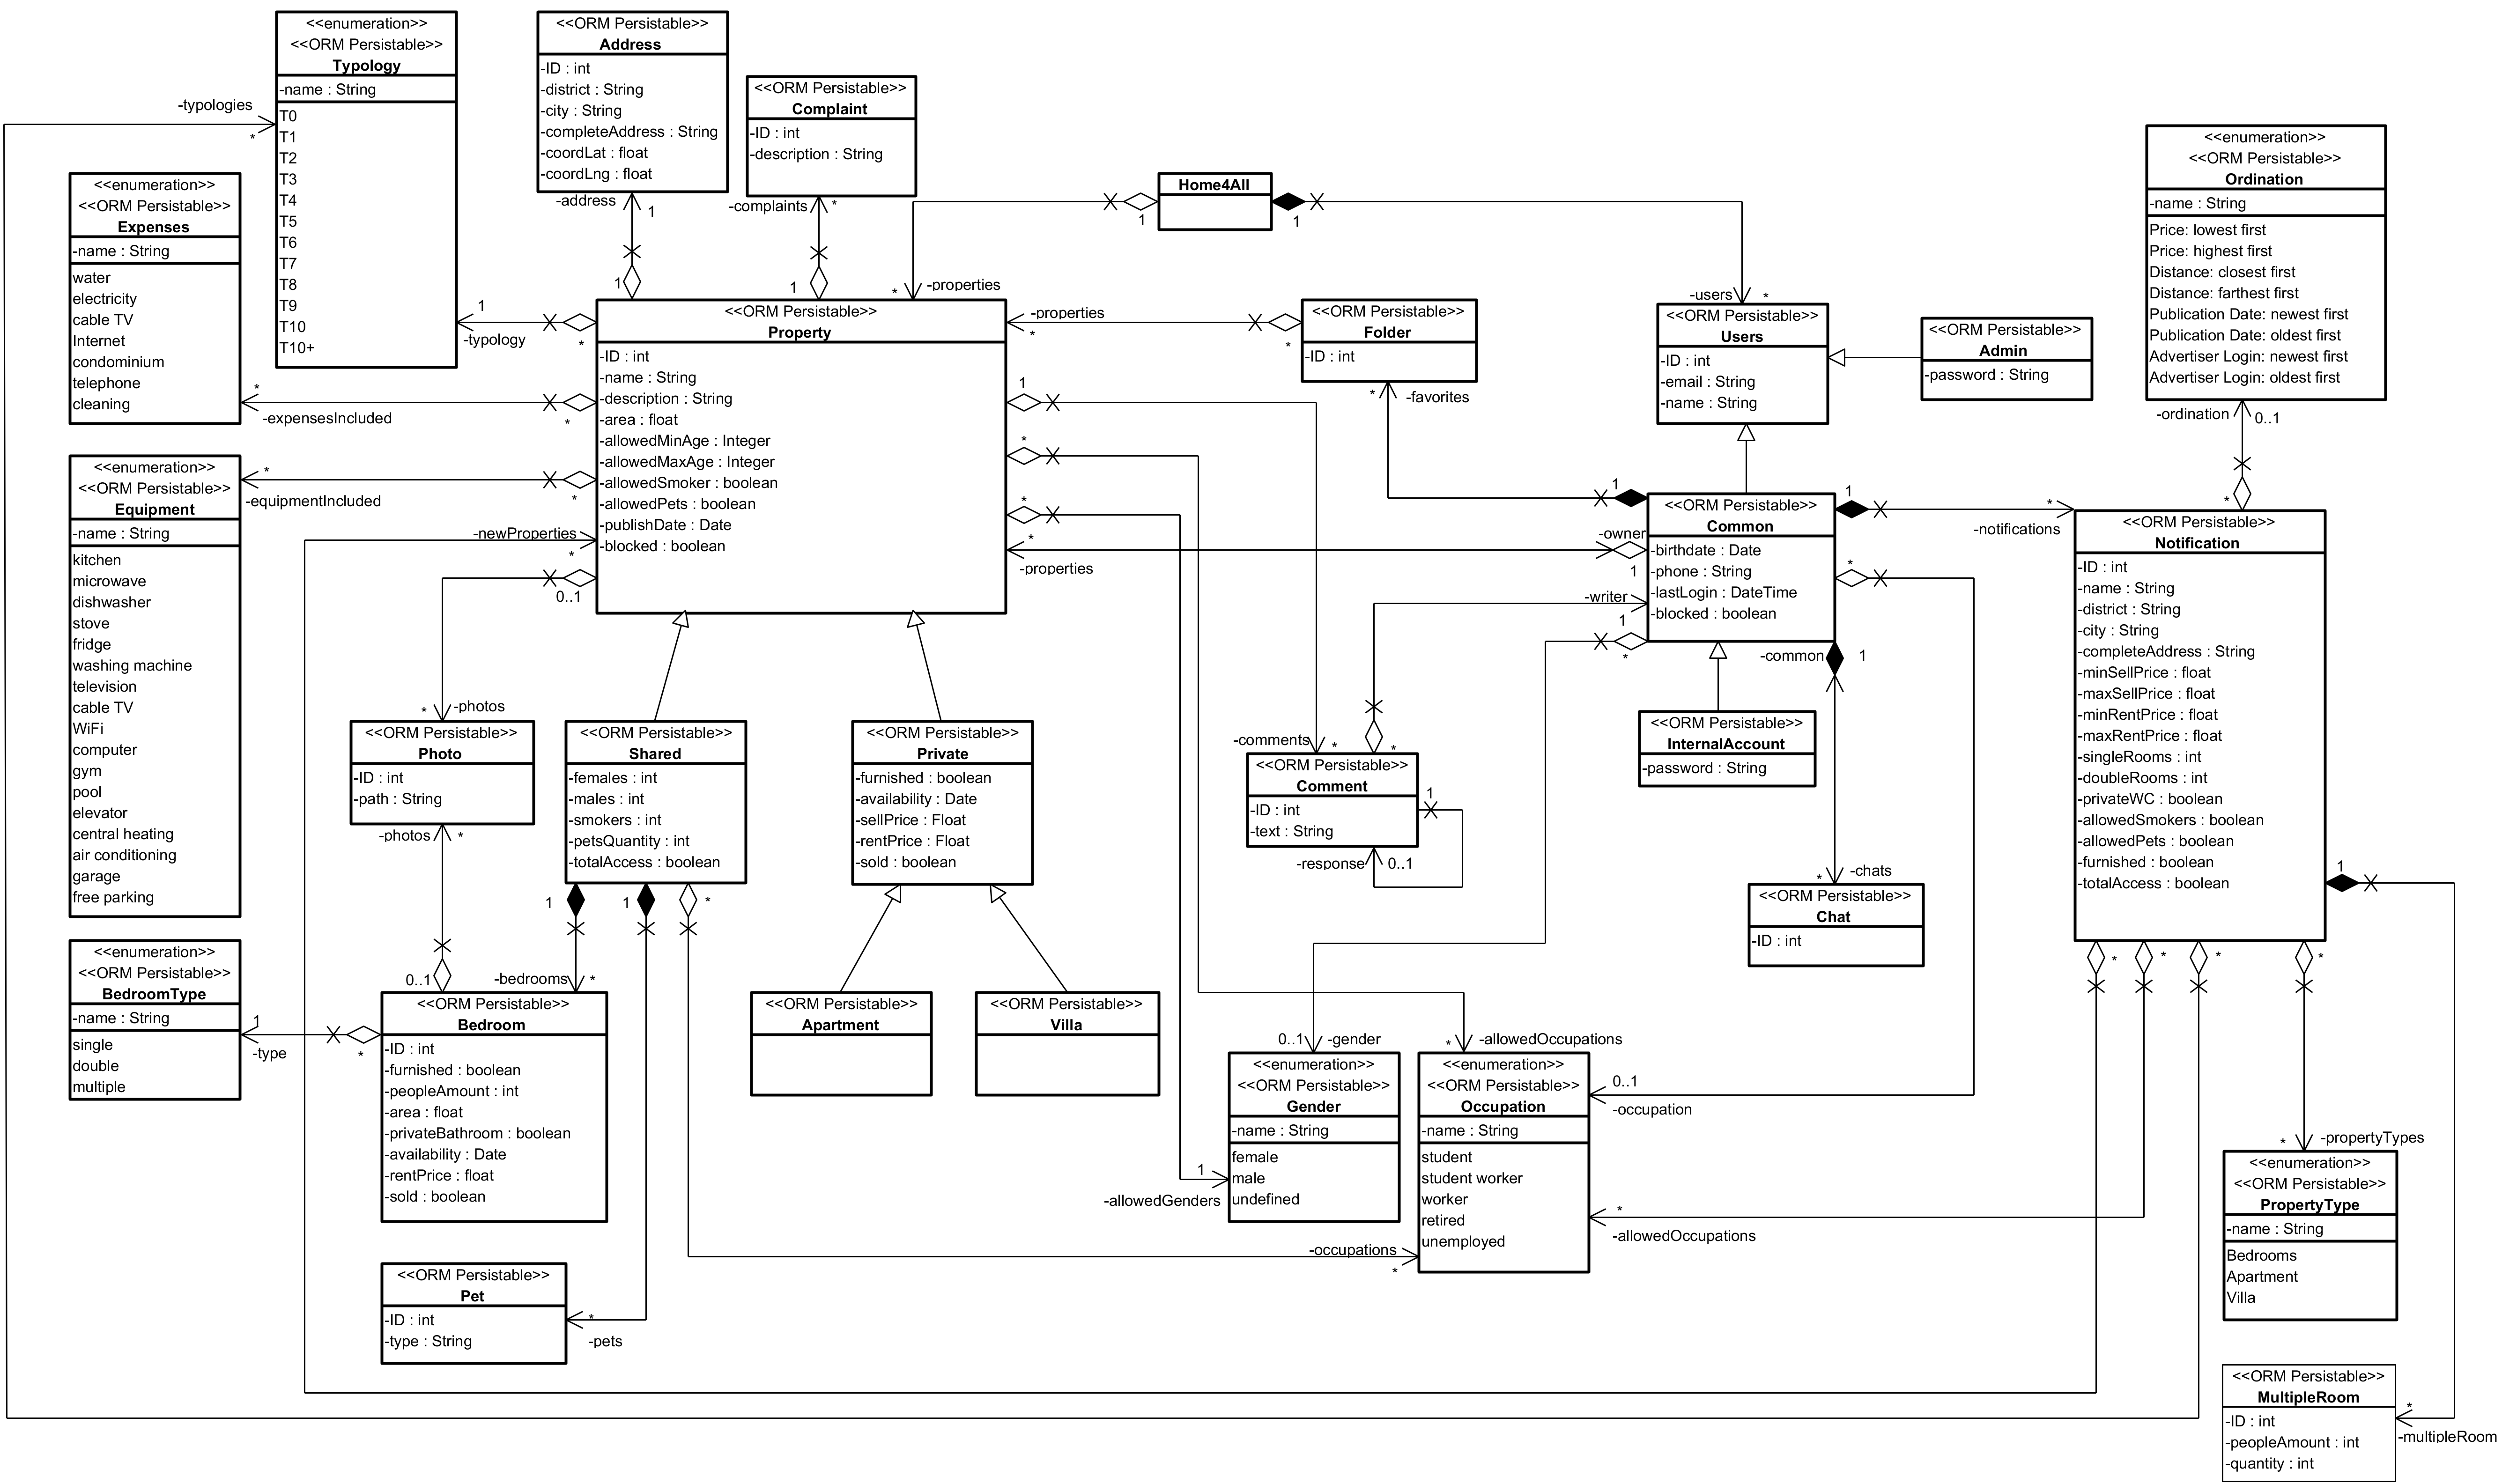
\includegraphics[width=1.6\textwidth]{images/PSM.png}
        \caption{Modelo dependente da tecnologia \texttt{Hibernate} para a aplicação \texttt{Home4All}.}
        \label{fig:psm_hibernate}
    \end{figure}
\end{landscape}

Relativamente à arquitetura final do projeto, com EJBs, organizou-se o mesmo em 3 \textit{packages} principais, sendo estes o \texttt{web}, o \texttt{business} e o \texttt{data}, referentes respetivamente à camada de apresentação, negócio e dados. O \textit{package} \texttt{business} contém uma \textit{Facade}, com o intiuto de simplificar o acesso aos \textit{Session Beans} contidos no \textit{package} \texttt{beans}. Os \textit{Session Beans}, por sua vez, acedem aos \textit{Entity Beans} presentes no \textit{package} \texttt{entities}. Esta arquitetura geral encontra-se representada no diagrama da figura \ref{fig:psm_general}, podendo consultar-se os detalhes referentes aos \textit{packages} \texttt{web}, \texttt{business} e \texttt{data} nas figuras \ref{fig:psm_presentation}, \ref{fig:psm_business} e \ref{fig:psm_data}, respetivamente.

\begin{figure}[H]
    \centering
    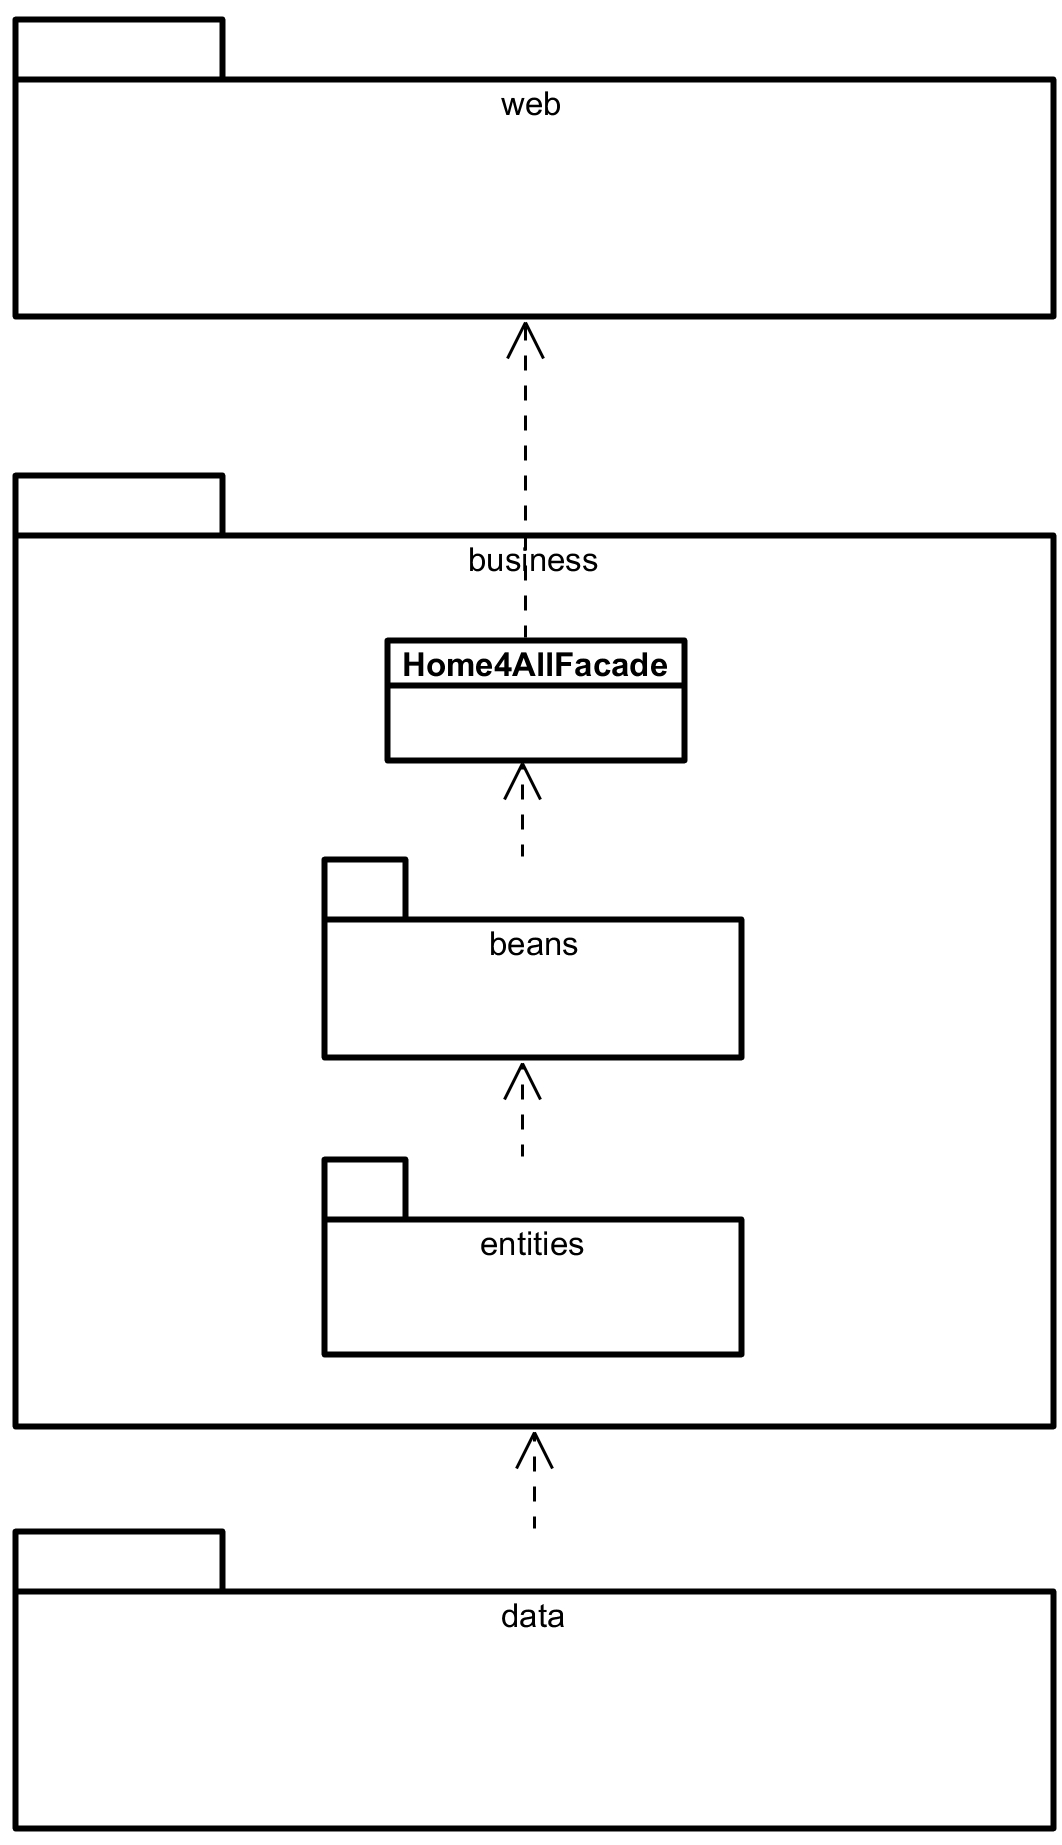
\includegraphics[width=0.6\textwidth]{images/PSM_General.png}
    \caption{Arquitetura geral da aplicação \texttt{Home4All}.}
    \label{fig:psm_general}
\end{figure}

\begin{figure}[H]
    \centering
    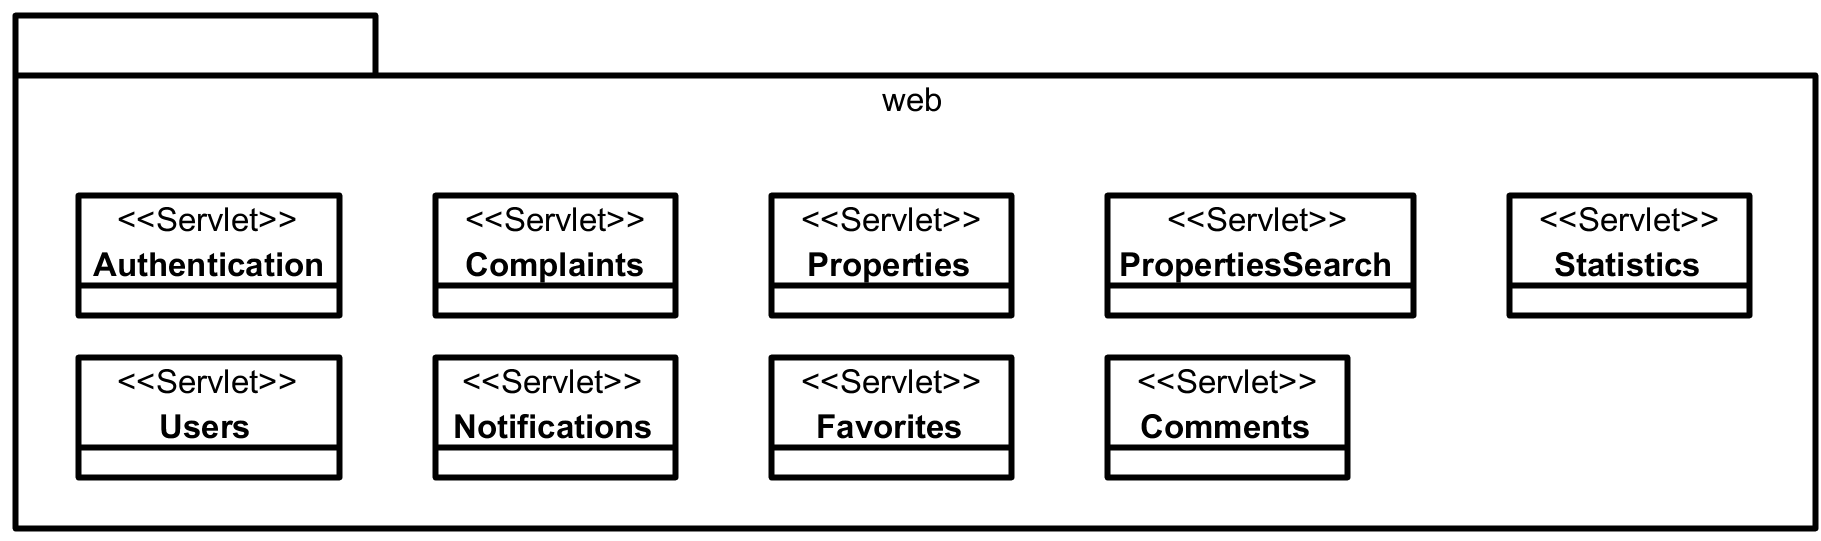
\includegraphics[width=\textwidth]{images/PSM_Presentation.png}
    \caption{Arquitetura da camada de apresentação da aplicação \texttt{Home4All} (\texttt{Servlets}).}
    \label{fig:psm_presentation}
\end{figure}

\begin{figure}[H]
    \centering
    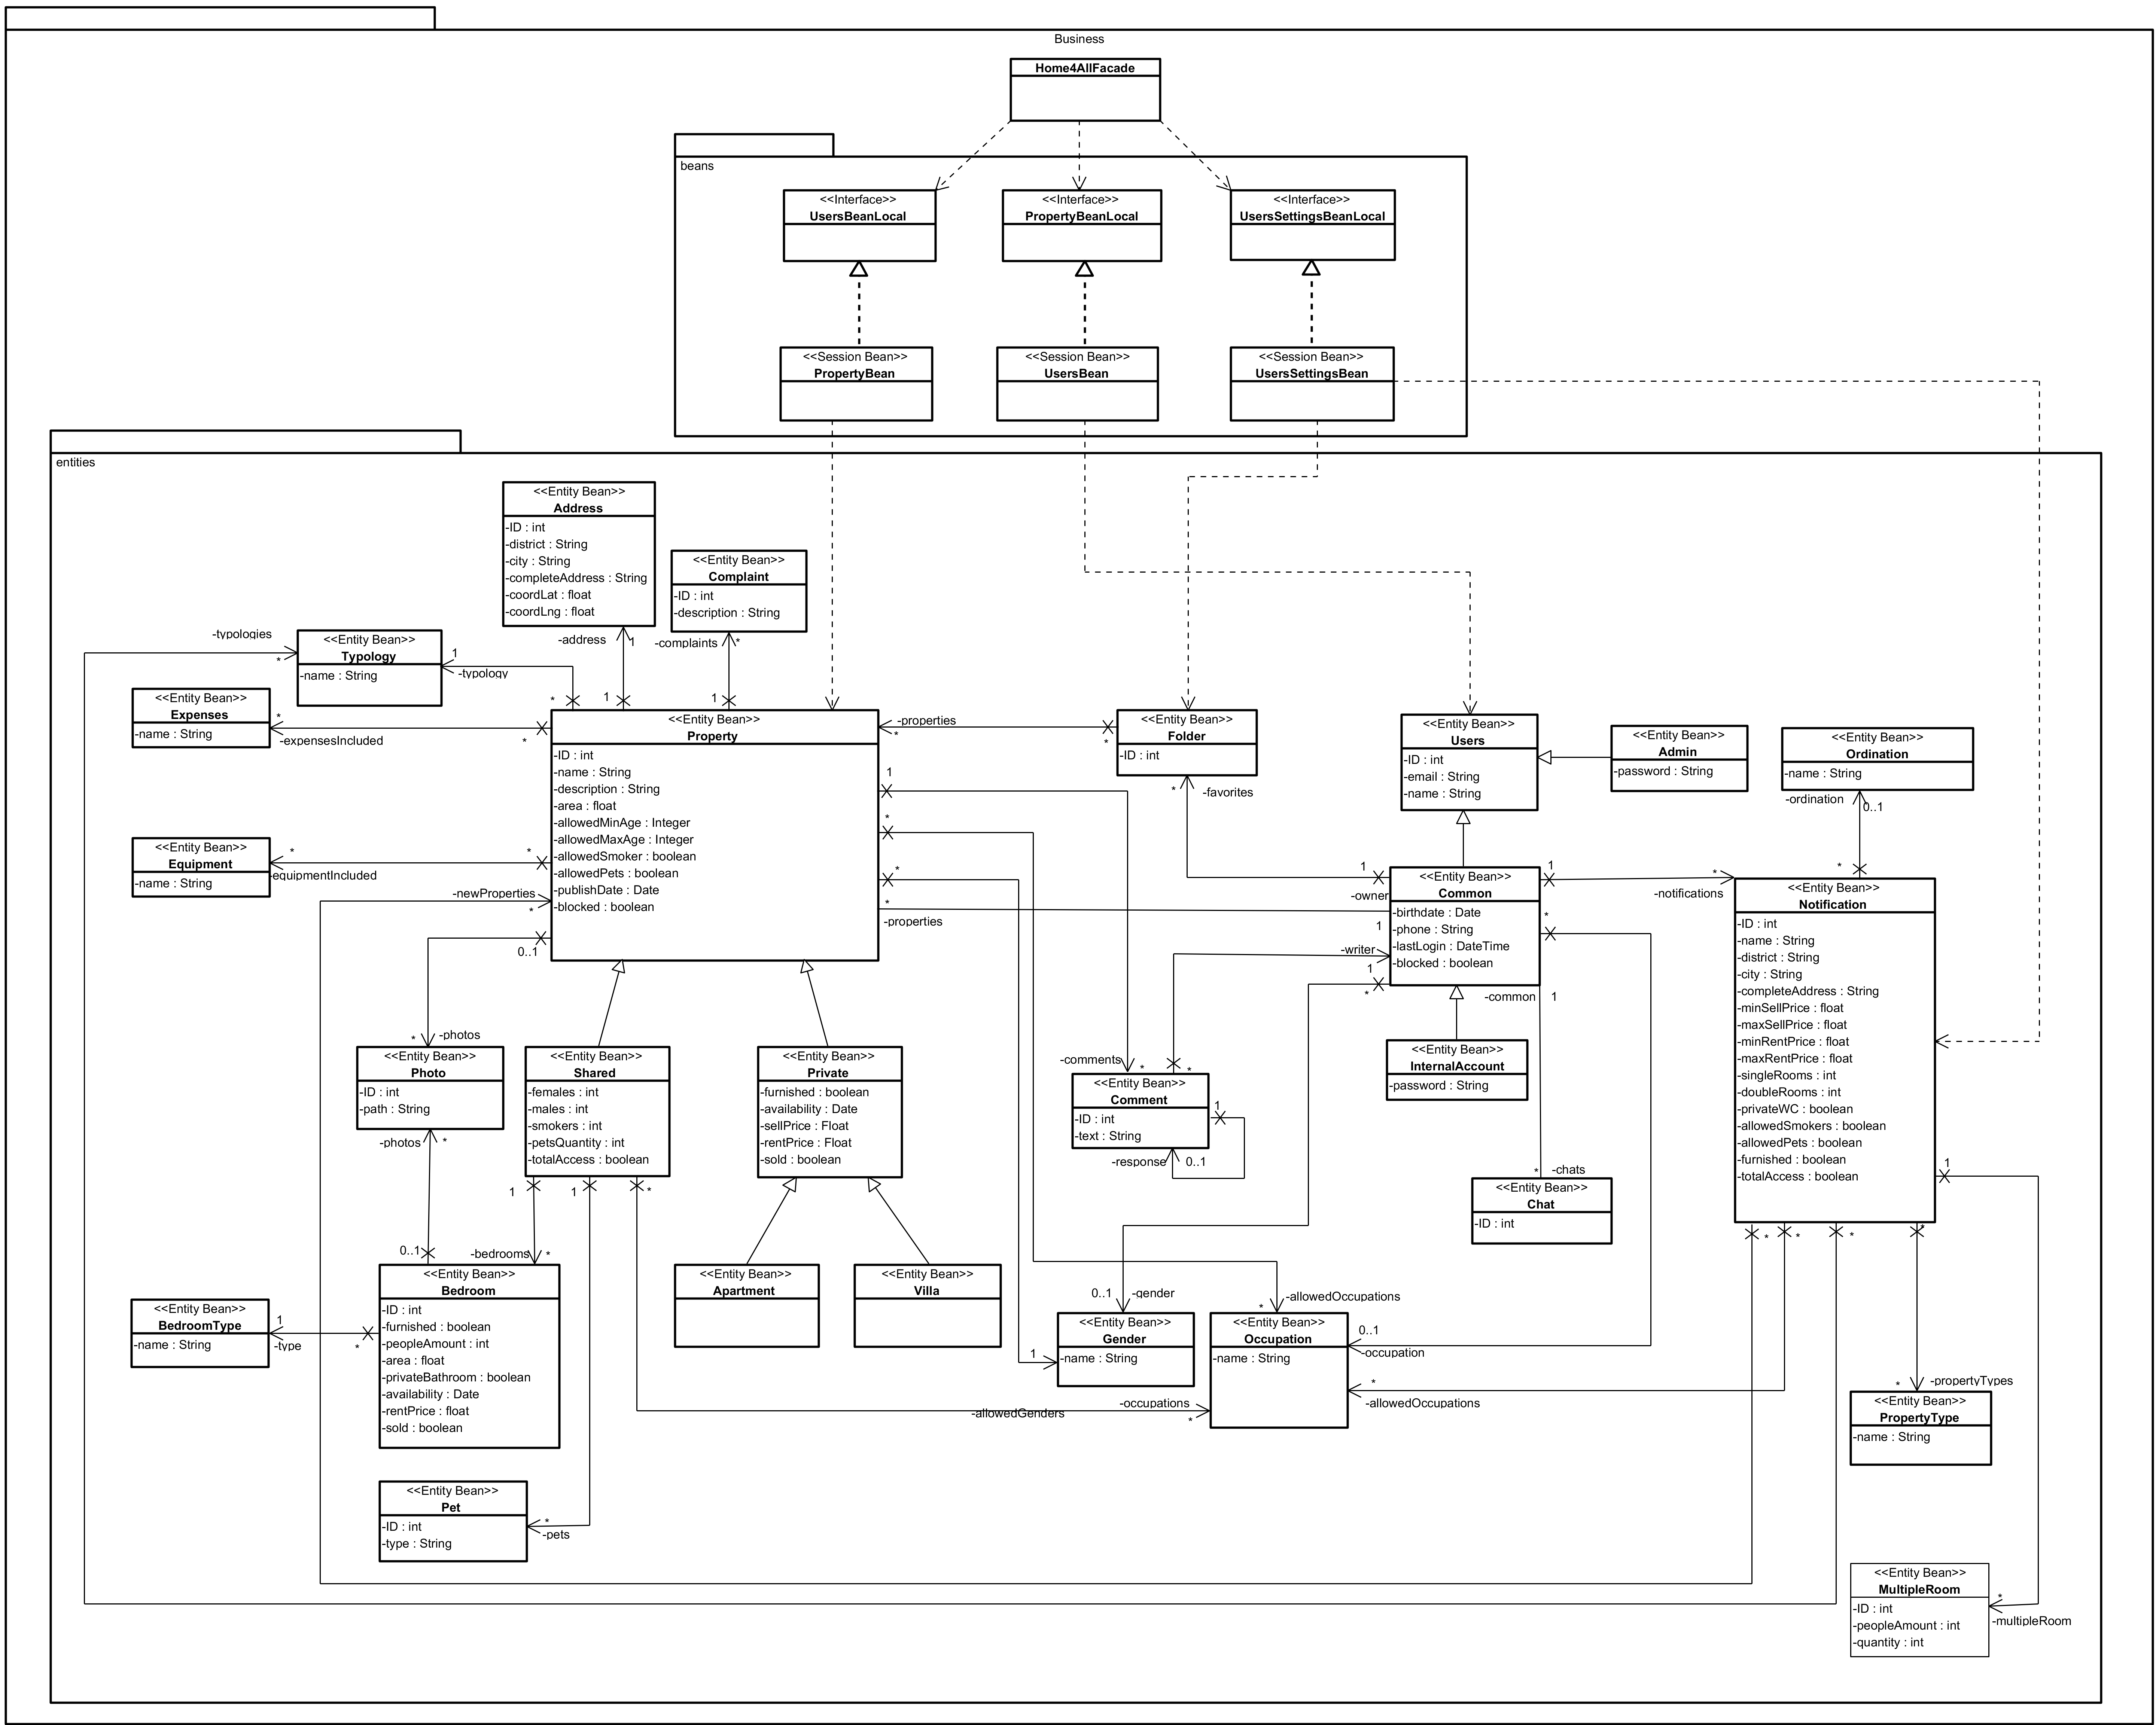
\includegraphics[width=1\textwidth]{images/PSM_Business.png}
    \caption{Arquitetura da camada de negócio da aplicação \texttt{Home4All} (\texttt{EJBs}).}
    \label{fig:psm_business}
\end{figure}

\begin{figure}[H]
    \centering
    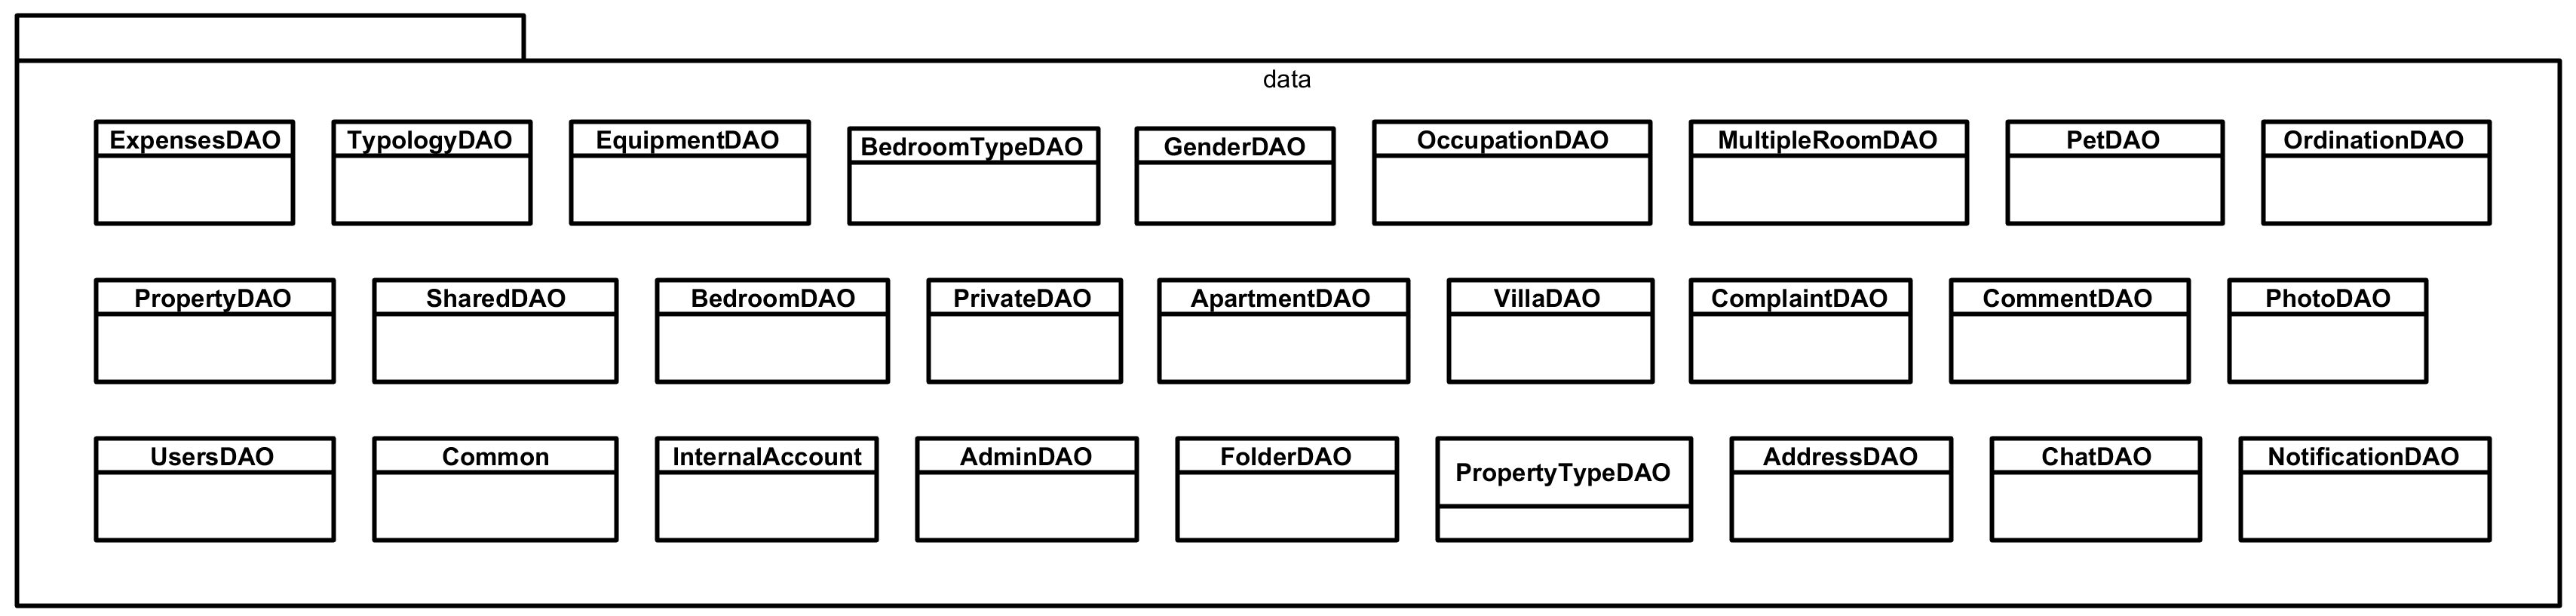
\includegraphics[width=1\textwidth]{images/PSM_Data.png}
    \caption{Arquitetura da camada de dados da aplicação \texttt{Home4All} (\texttt{DAOs}).}
    \label{fig:psm_data}
\end{figure}



\subsection{Implementação}


\subsubsection{Dificuldades encontradas e decisões mais importantes}
%- [ ] tecnologias: yarn, Google API, gravatar, samba
%- [ ] dificuldades nas queries dos filtros - utilização de queries nativas em vez de hql
%- [ ] Tratamento diferente dependente do tipo de propriedade
\paragraph{\textit{Frontend}}

Um dos desafios que o projeto \texttt{Home4All} coloca, está relacionado com a funcionalidade de pesquisa com base numa dada localização. Desta forma, poder-se-ia deixar que o utilizador escrevesse de forma livre a localização que pretendesse. No entanto, essa estratégia obrigava ao desenvolvimento de um motor de pesquisa, uma vez que a forma do utilizador inserir a mesma localização pode diferir. Assim sendo, foi necessário haver uma compromisso entre permitir que o utilizador escrevesse livremente ou selecionasse um conjunto de cidades já predefinido. Posto isto, a solução encontrada passa por utilizar a \texttt{API da Google} de \textit{autocomplete} de lugares para derivar as localizações que fazem \textit{match} com o que o utilizador se encontra a escrever de forma livre. Esta estratégia permite derivar a mesma informação caso diferentes utilizadores tentem escrever a mesma localização com ligeiras diferenças, mas acabem por escolher a mesma opção do \textit{autocomplete}. Consequentemente, o \textit{backend} apenas precisa de retornar os imóveis que fazem \textit{match} com uma das localizações, sem que exista a necessidade de computar complexos algoritmos de procura.

De realçar que, aparte do desafio mencionado anteriormente, o desenvolvimento do \textit{frontend} decorreu sem dificuldades de maior.

\paragraph{\textit{Backend}}
Quanto ao desenvolvimento do \textit{backend}, este foi realizado com o apoio dos diagramas de classes desenvolvidos, mais concretamente os apresentados nas figuras \ref{fig:psm_presentation}, \ref{fig:psm_business} e \ref{fig:psm_data}. 

Em termos de funcionalidades, a maior dificuldade encontrou-se no facto de diferentes tipos de propriedades(\texttt{Private} \textbf{vs} \texttt{Shared}) serem tratos de forma diferente em termos de pesquisa e dados associados. Assim, houve necessidade de dar um tratamento especial à imóvel \texttt{Private}, que inclui várias entidades que podem ser arrendadas (\texttt{Bedrooms}).

Para além disso, \textit{queries} mais complexas eram difíceis de escrever na linguagem HQL tendo-se optado nesses casos por escrever \textit{queries} nativas (SQL).

Outras dificuldades foram a obtenção de uma imagem representativa do utilizador autenticado e o armazenamento das fotografias dos imóveis.

Para o primeiro problema, optou-se pela utilização da API externa \texttt{Gravatar}, que permite o acesso a uma imagem definida pelo utilizador, através do seu email. Caso este não tenha associado uma imagem ao seu email, no \texttt{Gravatar}, é apresentada uma imagem por defeito.

Para o segundo problema, ponderou-se o armazenamento das imagens na base de dados. Contudo, chegou-se à conclusão de que esta técnica seria ineficiente, tendo em conta que a obtenção e armazenamento de imagens estariam sujeitos a mecanismos transacionais. Assim, optou-se por armazenar apenas o identificador da imagem na base de dados, e armazenar o próprio documento num sistema de ficheiros. A primeira solução explorada foi o \texttt{Samba}, que permite o armazenamento das imagens numa diretoria partilhada, num servidor de base de dados. Contudo, verificou-se que se obteria melhor desempenho utilizando a ferramenta \texttt{Redis}. Desta forma, foi esta ferramenta a escolhida como decisão final para o armazenamento das fotografias dos imóveis. 

\subsubsection{Funcionalidades implementadas}

Tendo em conta todas as dificuldades apresentadas durante o processo de desenvolvimento na secção acima, as funcionalidades inicialmente propostas não foram implementadas totalmente.

Assim, apresenta-se de seguida o diagrama de casos de uso em que se encontram representadas as funcionalidades implementadas na solução final.

\begin{document}
    \begin{figure}[!ht]
        \centering
        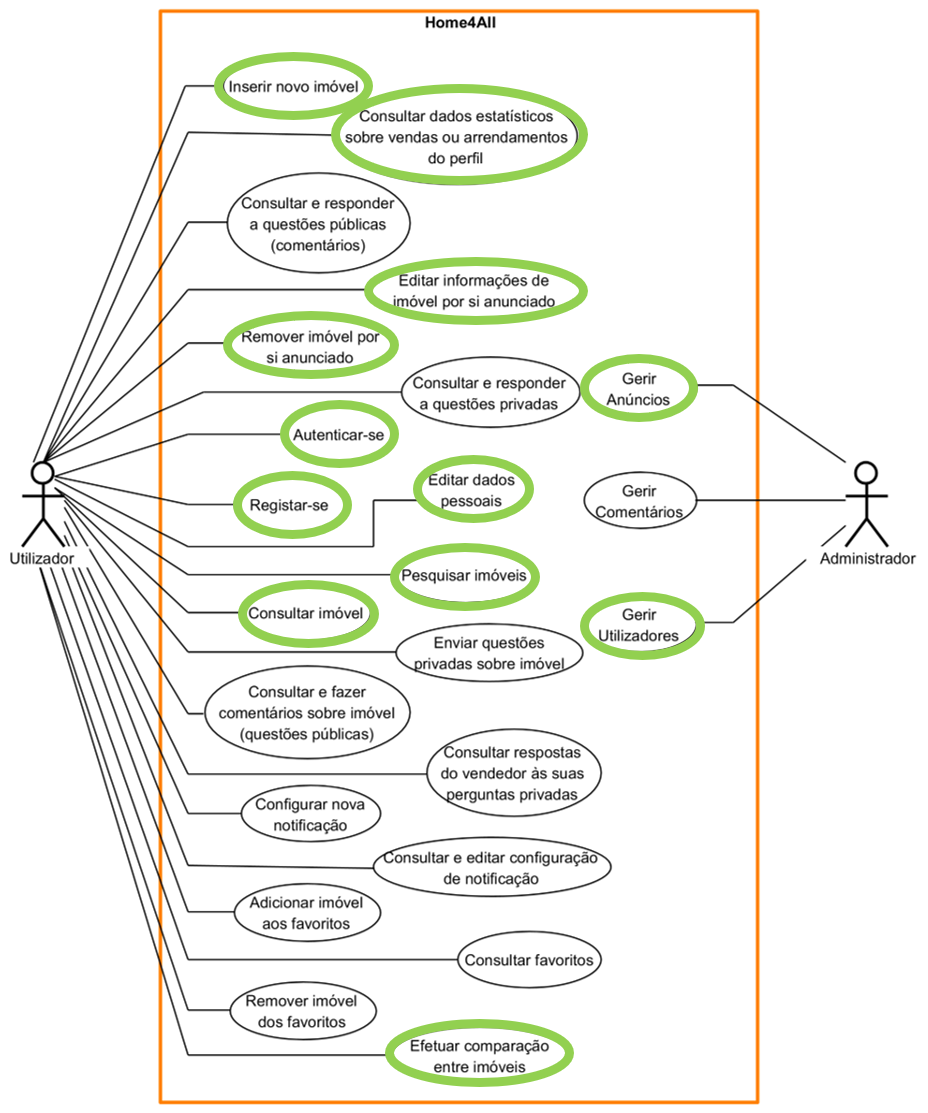
\includegraphics[width=0.6\textwidth]{images/Imagem1.png}
        \caption{Diagrama de casos de uso implementados na solução final.}
        \label{fig:diagrama_dominio}
    \end{figure}    
\end{document}

A ordem de implementação dos diversos casos de uso inicialmente propostos foi definida tendo em conta uma noção de prioridade inicialmente associada a cada caso de uso. Funcionalidades como a autenticação de um utilizador ou o seu registo, são essenciais para a integridade do sistema, tendo sido assim estas as primeiras a serem implementadas. Da mesma forma, casos de uso que a sua não implementação faça com que o produto apresentado perca totalmente o seu propósito, foram também priorizados. Por exemplo, a gestão de anúncios, pesquisa de imóveis e a comparação encontram-se diretamente relacionados com funcionalidades básicas de uma plataforma de imóveis pelo que foram considerados prioritários também em relação aos restantes casos de uso.

Em suma, todas as funcionalidades diretamente relacionadas com imóveis encontram-se implementadas, ficando apenas em falta funcionalidades que apenas tornariam o contacto entre anunciante e cliente mais simples e rápido.


\subsubsection{Interface de utilizador}

Para o desenvolvimento da camada de apresentação da plataforma, foram tidos como base os \textit{mockups} anteriormente desenhados. Assim, numa fase inicial a construção da interface foi principalmente orientada à funcionalidade e não tanto à sua apresentação. De seguida, passou-se então à personalização dos componentes para que a apresentação ficasse o mais parecida possível com os \textit{mockups}.

Assim, apresenta-se a interface desenhada para o utilizador.

\begin{figure}[htb]
\centering
    \begin{subfigure}[h]{0.39\textwidth}
        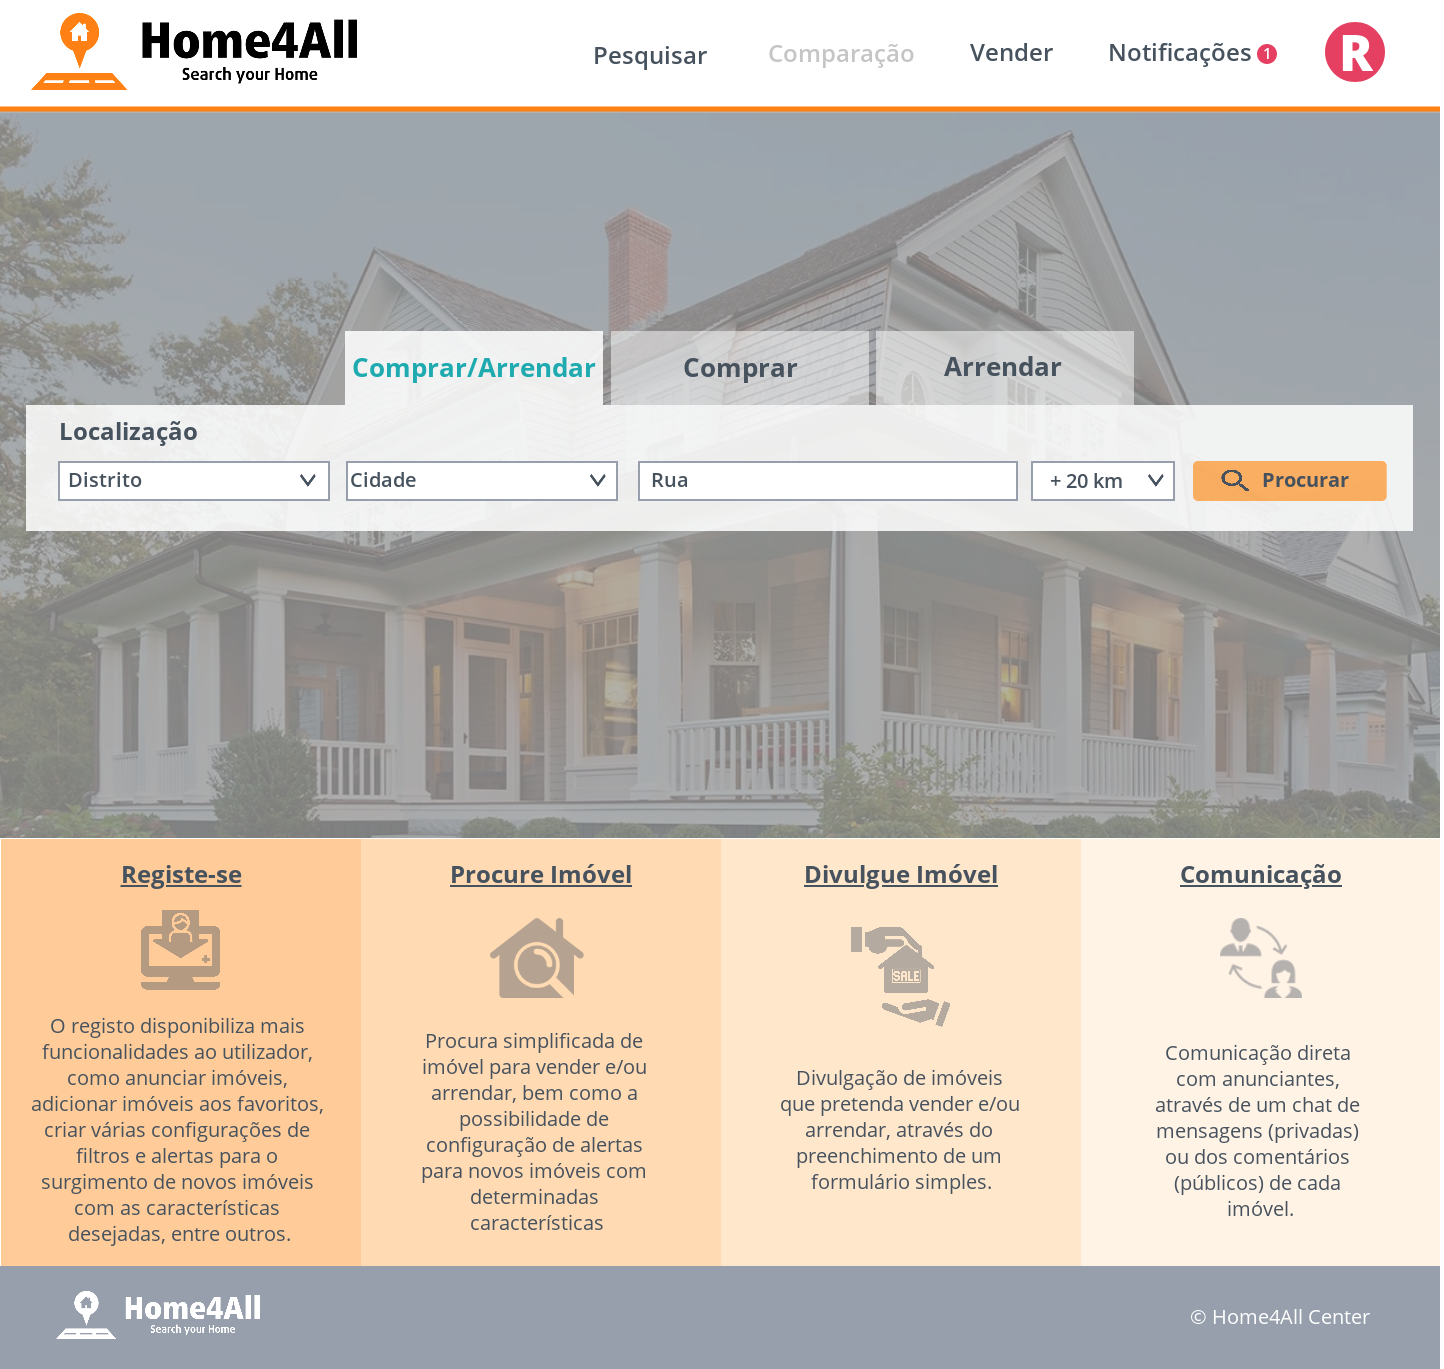
\includegraphics[width=\textwidth]{images/UI/Home_Login.png}
        \caption{Mockup.}
        \label{fig:fig1}
    \end{subfigure}
        \begin{subfigure}[h]{0.6\textwidth}
        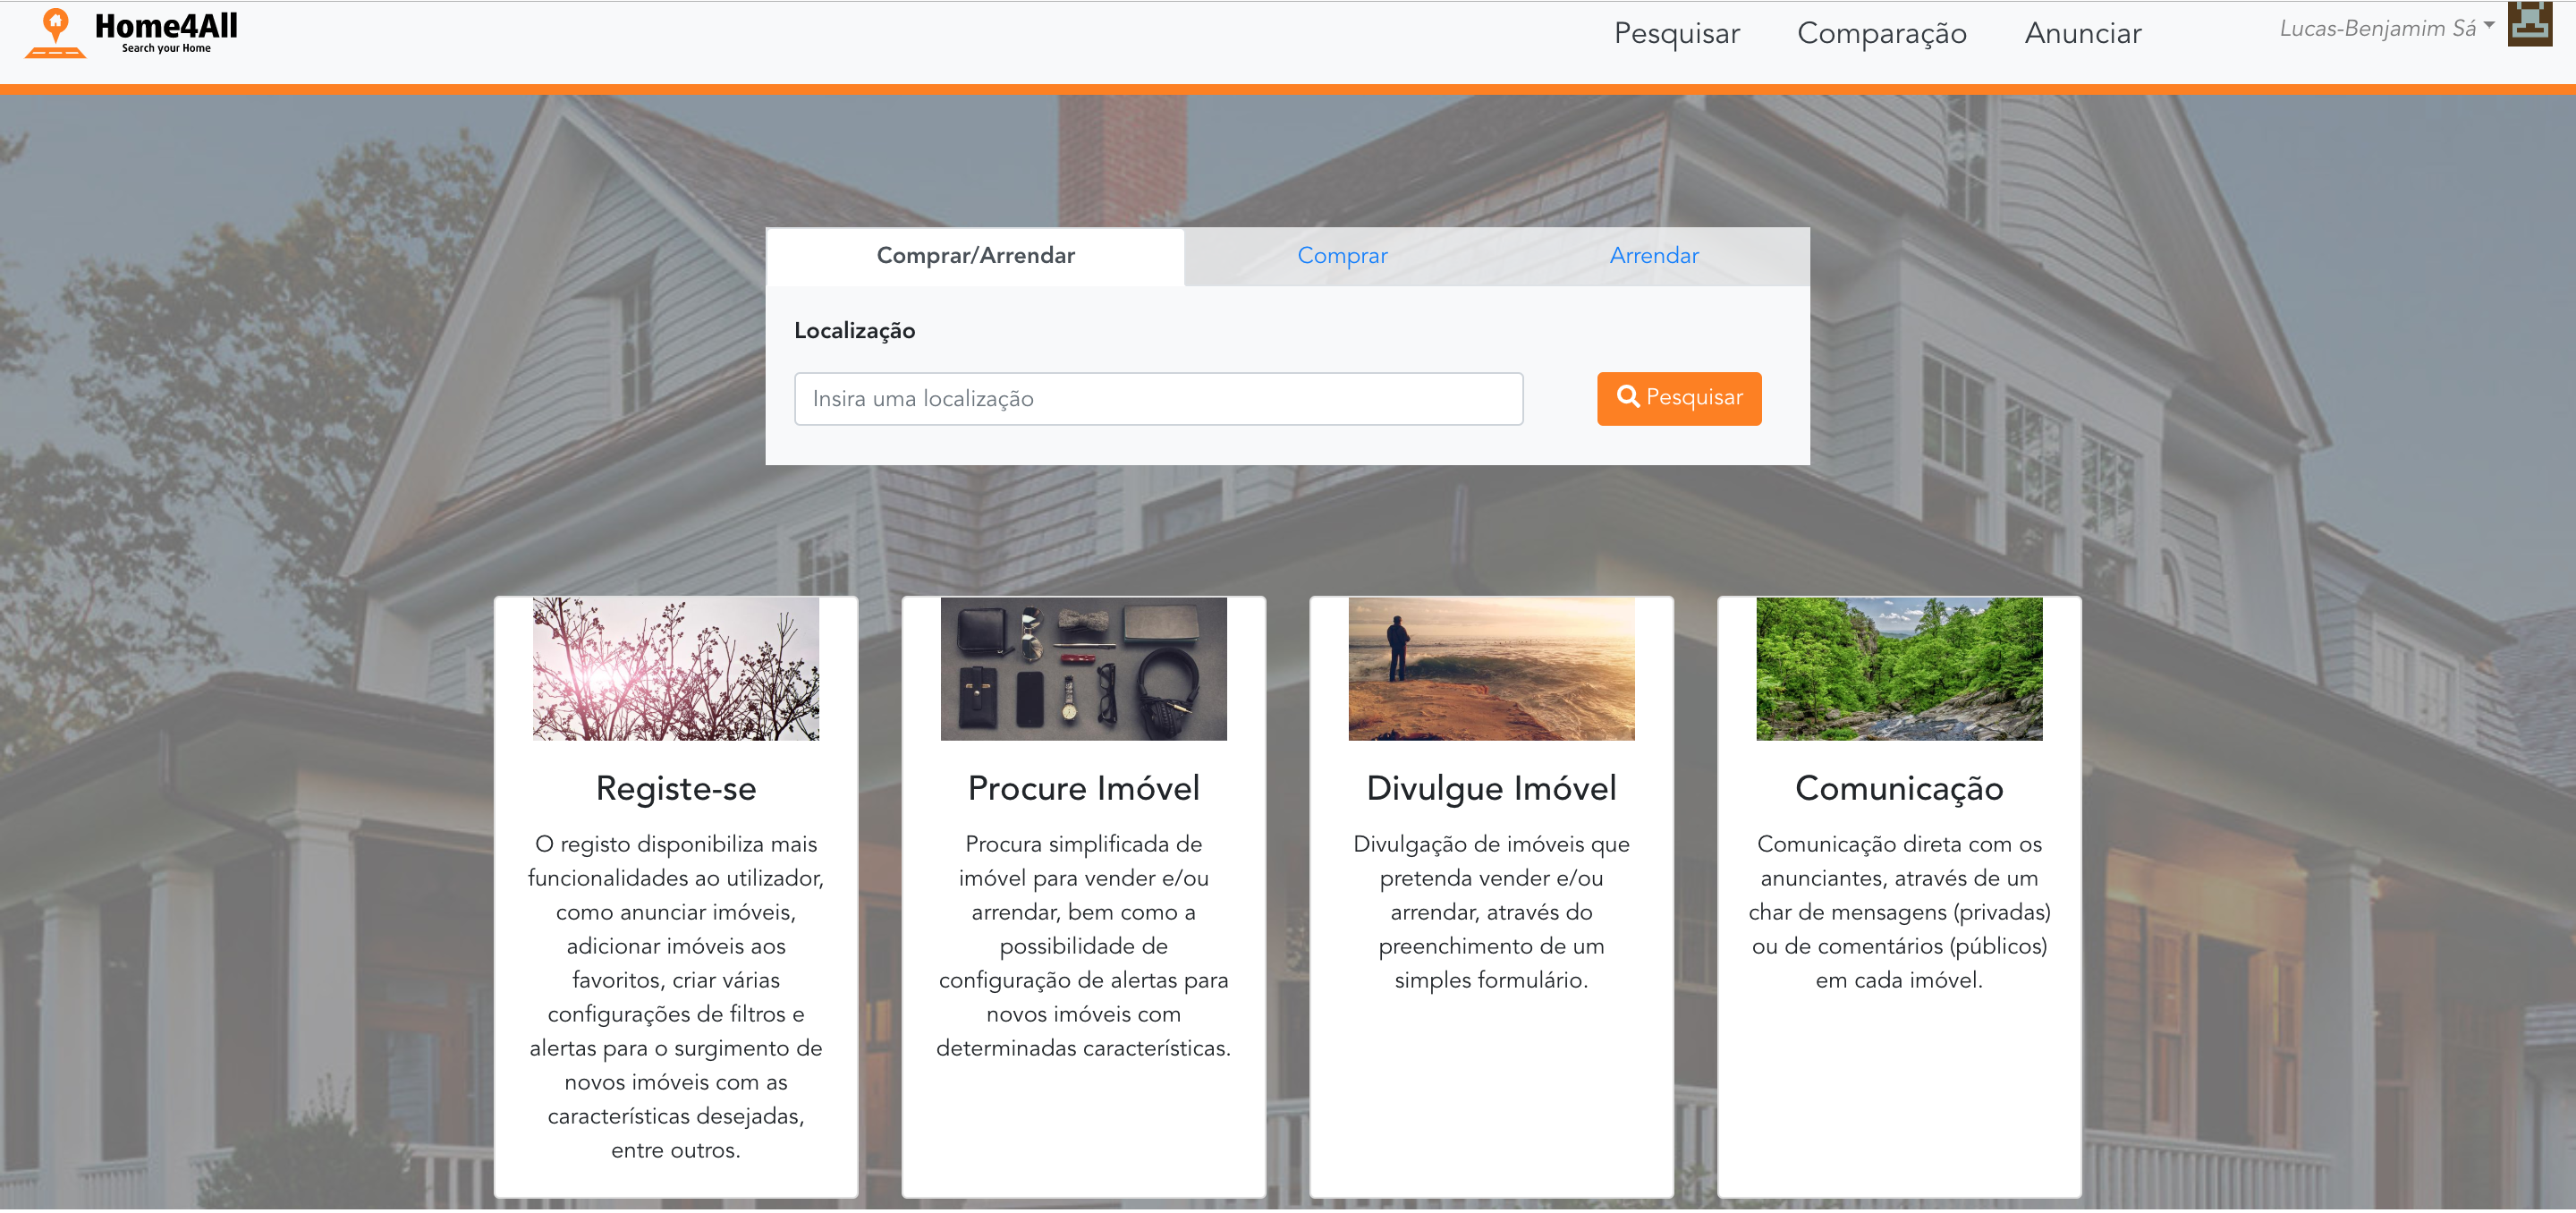
\includegraphics[width=\textwidth]{images/UI/home-real.png}
        \caption{Implementação}
        \label{fig:fig2}
    \end{subfigure}
\caption{Comparação entre \textit{mockup} e implementação.}
\label{fig:subfigureexample}
\end{figure}

Como se pode observar, o resultado final encontra-se bastante próximo do que foi inicialmente idealizado.

Outra das páginas a analisar será a visualização das informações do perfil. Neste caso, o resultado final não foi o mais fiel aos \textit{mockups} desenvolvidos tendo em conta que a apresentação dos campos de informação na versão original não apresenta apenas um campo de informação por linha, enquanto que na versão implementada é esse o caso.

Vejam-se então as duas versões da interface.

\begin{figure}[htb]
\centering
    \begin{subfigure}[h]{0.5\textwidth}
        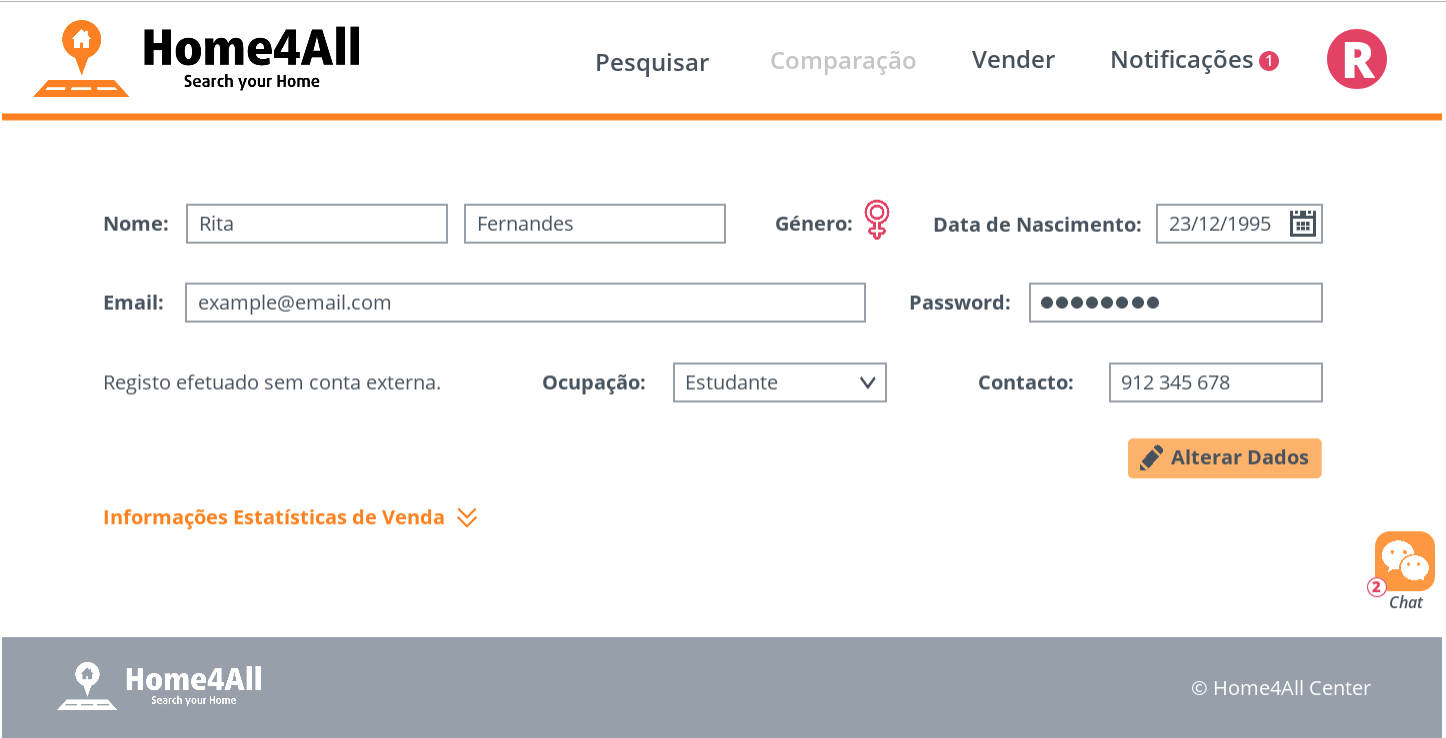
\includegraphics[width=\textwidth]{images/UI/PersonalInfo.png}
        \caption{Mockup.}
        \label{fig:fig1}
    \end{subfigure}
    \begin{subfigure}[h]{0.49\textwidth}
        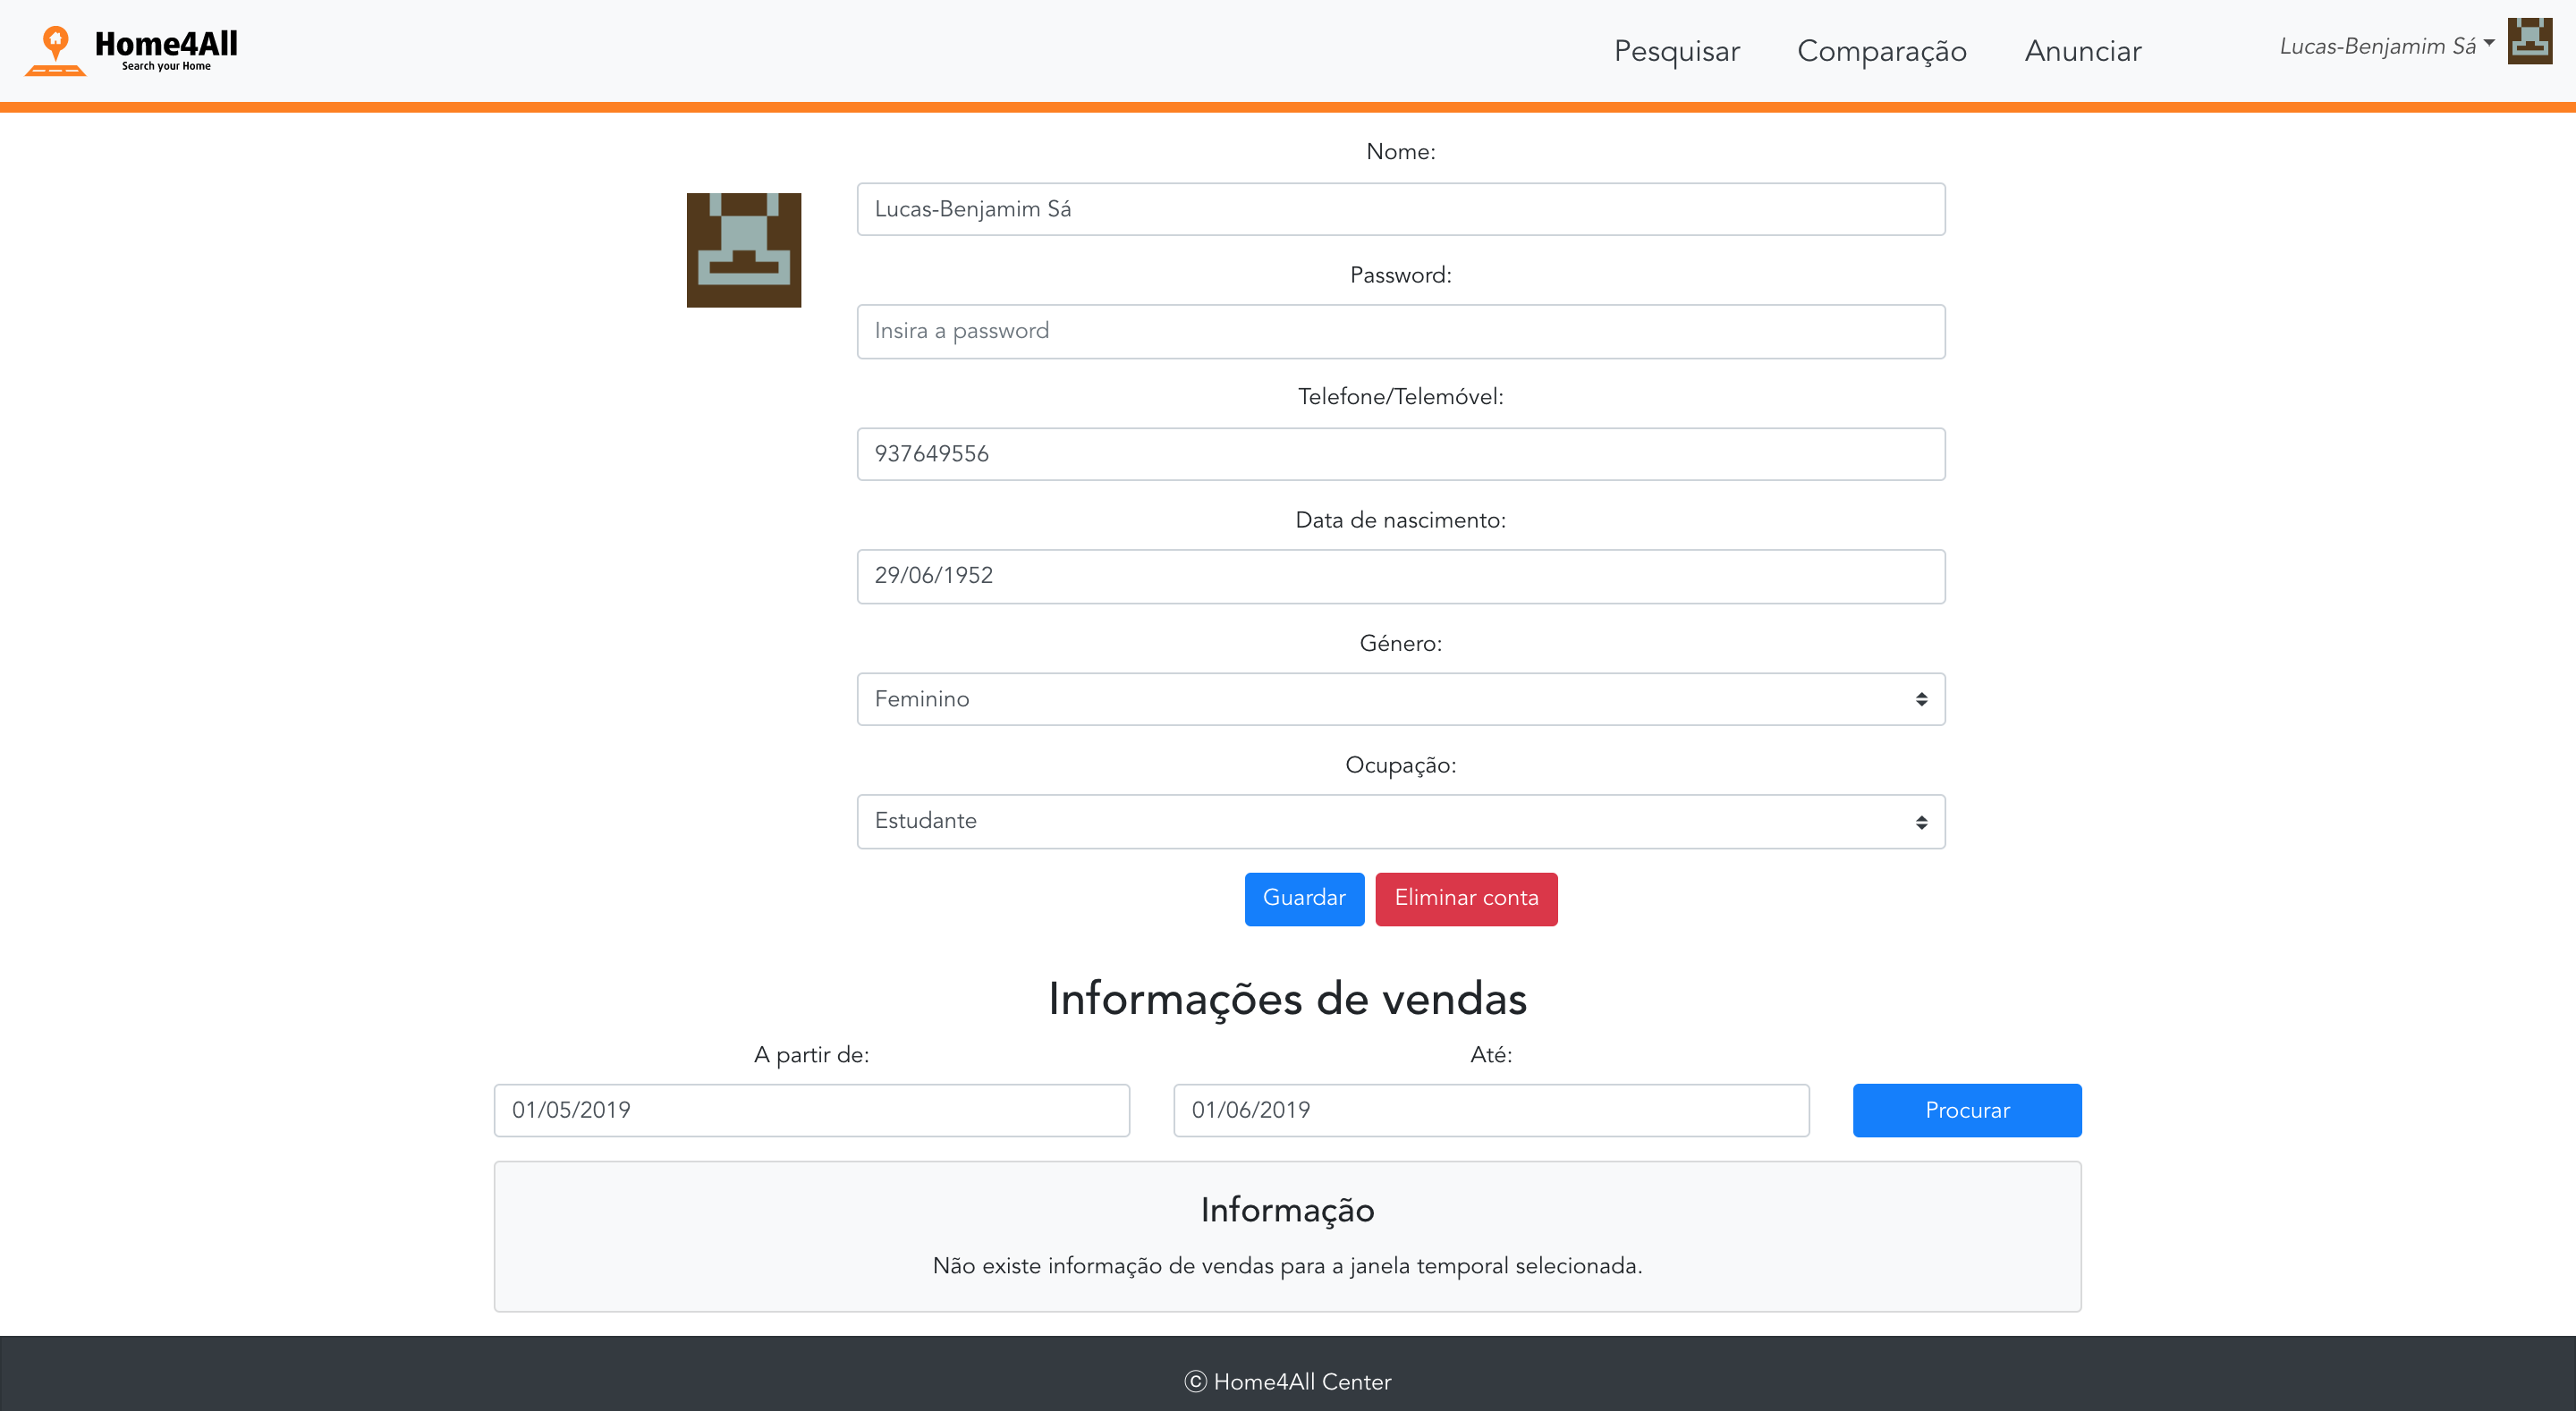
\includegraphics[width=\textwidth]{images/UI/userInfo-real.png}
        \caption{Implementação}
        \label{fig:fig2}
    \end{subfigure}
\caption{Comparação entre \textit{mockup} e implementação.}
\label{fig:subfigureexample}
\end{figure}

De uma forma geral, todas as páginas seguiram praticamente a 100\% o aspeto dos \textit{mockups} anteriormente desenvolvidos. A única diferença considerável entre a versão previamente desenhada e a versão final será mesmo a página de visualização da informação do perfil.


\newpage
\section{\textit{Deployment}}

Após a implementação do projeto \texttt{Home4All}, torna-se necessário fazer o \textit{deployment} do mesmo, de forma a que este possa ser usado e testado em situações reais. Deste modo, é imperativo que se analise a melhor estratégia de forma a tirar o máximo proveito dos recursos disponíveis, garantindo elevada disponibilidade, assim como tempos de resposta aceitáveis.

Assim sendo, dado que se trata de uma aplicação \textit{web}, é comum que esta contenha um servidor \textit{web}, um servidor aplicacional e um camada de dados. Na prática esta ferramenta utiliza como \textit{web server} o \texttt{Apache}. Para que o \textit{website} seja servido, foi necessário compilar o projeto de \textit{front-end} em \texttt{Vuejs} para o modo de produção e coloca-lo na diretoria apropriada do \texttt{Apache} para que este ficasse disponível. Além disso, dado que o servidor \textit{web} é o primeiro ponto de entrada no sistema, decisões tomadas neste ponto podem ser decisivas para o desempenho do sistema. Como tal, houve o cuidado de configurar o servidor para que este permitisse balançar a carga pelos servidores aplicacionais existentes. No entanto, um simples balanceamento poderia comprometer o conceito de sessão utilizado na componente aplicacional da ferramenta. Efetivamente, mecanismos de \textit{cache} ou mesmo a gestão de informação relacionada com a sessão do utilizador ficariam perdidos caso o utilizador fosse balanceado para diferentes servidores aplicacionais numa mesma utilização. Por um lado, uma possível estratégia seria sincronizar em tempo real essas informações entre os diversos servidores aplicacionais. Por outro lado, pode-se configurar o servidor \textit{web} para que identifique cada sessão de utilizador e garanta, que após inicializada, é sempre servida pelo mesmo servidor aplicacional. Neste projeto em concreto foi escolhida a segunda opção uma vez que diminui a carga necessária para a sincronização dos servidores aplicacionais. Além disso, é na mesma possível realizar o balanceamento dos pedidos recebidos,  sendo que agora este processo encontra-se associado ao conceito de sessão.

Após a configuração dos servidores \textit{web} os clientes possuem acesso ao conteúdo estático do \textit{website}, e como tal, conseguem navegar em grande parte do \textit{website}. No entanto, os pedidos realizados ao \textit{backend} são redirecionados pelo \textit{web server}, mas não obtêm qualquer resposta. Desta forma, torna-se necessário configurar os servidores aplicacionais que vão permitir animar a lógica associado à aplicação Home4All e assim devolver ao cliente os dados que este necessita para utilizar a ferramenta na sua plenitude. Este processo foi alcançado através da utilização do servidor aplicacional \texttt{Wildfly}. Este é responsável por receber aos pedidos HTTP reencaminhados pelo \texttt{Apache} e fornecê-los ao \textit{servlet} respetivo do JEE. Da mesma forma, quando o pedido em está pronto a ser enviado, este realiza o percurso contrário de forma a fazer chegar ao cliente os dados requeridos. 

Sendo a camada aplicacional independente da camada dos dados assim como da camada da apresentação, é possível fazer \textit{deploy} da mesma, de forma isolada dos restantes componentes. Assim sendo, a estratégia utilizada passou por gerar um ficheiro WAR da camada aplicacional, de forma a que este contenha todas as bibliotecas necessárias (e.g. \texttt{Hibernate}), assim como o servidor aplicacional anteriormente referido, de forma a que a camada se encontre completamente funcional. Após a geração do ficheiro, optou-se por executá-lo num \textit{container docker}, para que este tirasse partido das vantagens dessa tecnologia, nomeadamente no que toca à portabilidade associada à facilidade de realizar o \textit{deploy} em diferentes máquinas, utilizando o mesmo processo.

Por fim, tem-se a infraestrutura da aplicação praticamente operacional, restando apenas a camada de dados. O \textit{deploy} desta última consistiu na inicialização do servidor de \texttt{PostgreSQL} e do \texttt{Redis}. Após estas operações tem-se a estrutura final da aplicação montada e pronta a ser utilizada pelos clientes finais.



%%%%%%%%%%%%%%%%%%%%%%%%%%%%%%%%%%

\newpage
\section{Carga aplicacional}
\subfile{sections/dTestesCarga}

%%%%%%%%%%%%%%%%%%%%%%%%%%%%%%%%%%

\newpage
\section{Testes de usabilidade da interface}

Por forma a avaliar a qualidade da interface desenvolvida para a plataforma, foram realizados testes de usabilidade com base na execução de determinadas tarefas na plataforma.

De seguida, apresentam-se então em baixo os resultados dos testes realizados e as taxas de completude das tarefas a realizar respetivamente.

\begin{table}[H]
\centering
\caption{Resultados do questionário SUS recolhidos e respetivos \textit{scores}.}
\begin{tabular}{ccccccccccc}
\hline
\rowcolor[HTML]{EFEFEF} 
\textbf{1} & \textbf{2} & \textbf{3} & \textbf{4} & \textbf{5} & \textbf{6} & \textbf{7} & \textbf{8} & \textbf{9} & \textbf{10} & \textbf{TOTAL} \\ \hline
5          & 1          & 4          & 1          & 5          & 4          & 5          & 1          & 5          & 1           & 90             \\
4          & 1          & 4          & 1          & 4          & 1          & 5          & 1          & 4          & 1           & 90             \\
4          & 1          & 4          & 1          & 4          & 3          & 4          & 2          & 3          & 1           & 77,5           \\
5          & 2          & 5          & 1          & 5          & 1          & 5          & 2          & 4          & 1           & 92.5           \\ \hline
\end{tabular}
\end{table}

\begin{table}[H]
\centering
\caption{Resultados da completude das tarefas realizadas durante os testes e respetivos \textit{scores}.}
\begin{tabular}{ccccc}
\hline
\rowcolor[HTML]{EFEFEF} 
\textbf{1} & \textbf{2} & \textbf{3} & \textbf{4} & \textbf{TOTAL} \\ \hline
1          & 1          & 1          & 1          & 100\%          \\
1          & 1          & 1          & 1          & 100\%          \\
1          & 1          & 0,5        & 1          & 88\%           \\
1          & 1          & 1          & 1          & 100\%          \\ \hline
\end{tabular}
\end{table}

Através da observação dos resultados acima, conclui-se que a interface com o utilizador tem ainda alguns pontos a rever. Ainda assim, consideram-se positivos os resultados obtidos.